\documentclass[11pt,border=2pt]{standalone}
\usepackage{tikz}
\usetikzlibrary{arrows.meta,positioning}
\definecolor{bluebox}{HTML}{EAF2F8}
\definecolor{greenbox}{HTML}{EAF6EE}
\definecolor{goldbox}{HTML}{FFF4D6}
\definecolor{linegray}{HTML}{65737E}
\begin{document}
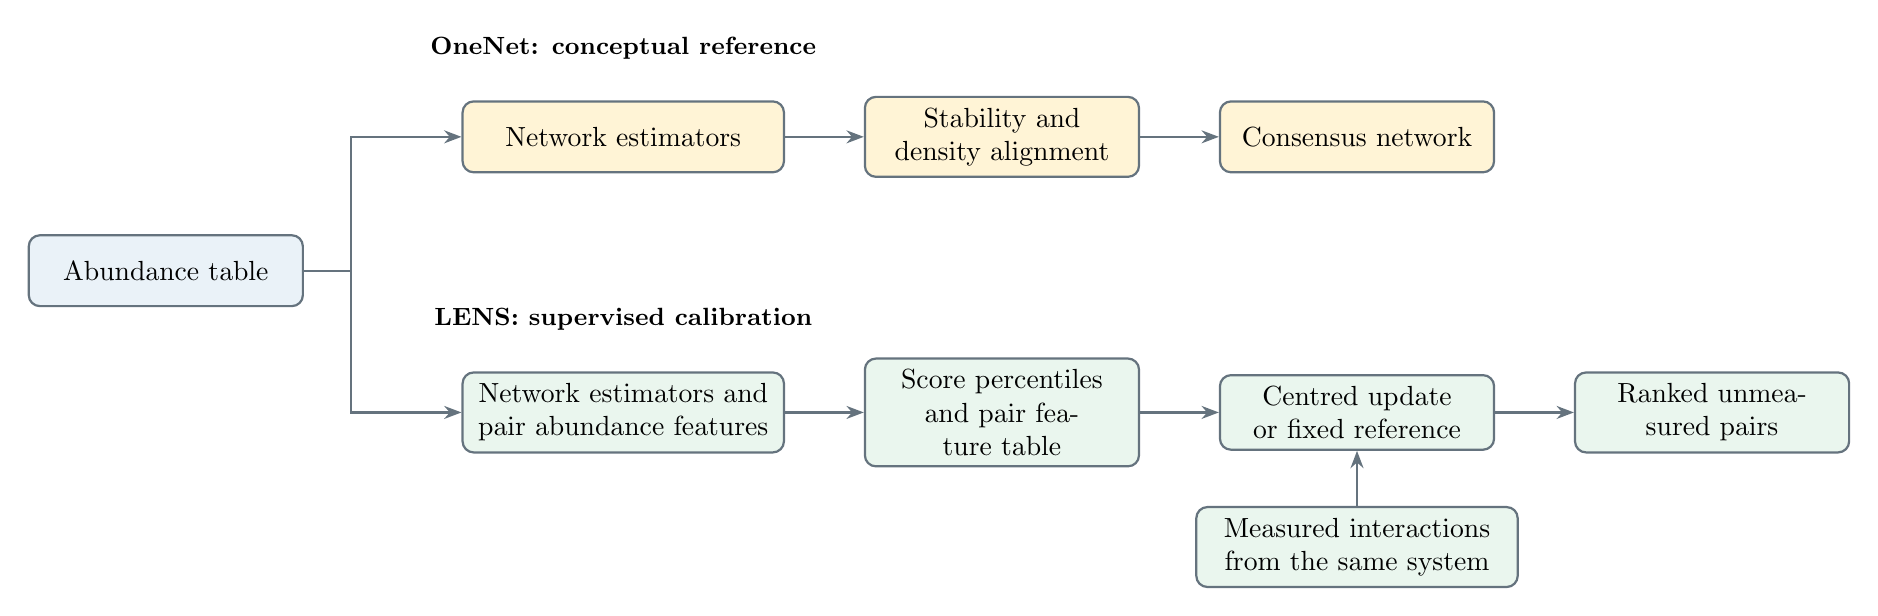
\begin{tikzpicture}[
  node distance=7mm and 10mm,
  box/.style={rounded corners, draw=linegray, thick, align=center, minimum height=9mm, text width=32mm, inner sep=4pt},
  common/.style={box, fill=bluebox},
  one/.style={box, fill=goldbox},
  sup/.style={box, fill=greenbox},
  arr/.style={-{Stealth[length=2.2mm]}, thick, draw=linegray},
  group/.style={font=\small\bfseries, align=center}
]
\node[common] (abund) {Abundance table};

\node[one, right=20mm of abund, yshift=17mm, text width=38mm] (oneestim) {Network estimators};
\node[one, right=of oneestim] (stability) {Stability and density alignment};
\node[one, right=of stability] (consensus) {Consensus network};
\node[group, above=4mm of oneestim] (onetitle) {OneNet: conceptual reference};
\draw[arr] (abund.east) -- ++(6mm,0) |- (oneestim.west);
\draw[arr] (oneestim) -- (stability);
\draw[arr] (stability) -- (consensus);

\node[sup, right=20mm of abund, yshift=-18mm, text width=38mm] (supestim) {Network estimators and pair abundance features};
\node[sup, right=of supestim] (scores) {Score percentiles and pair feature table};
\node[sup, right=of scores] (cal) {Centred update or fixed reference};
\node[sup, right=of cal] (prob) {Ranked unmeasured pairs};
\node[sup, below=of cal, text width=38mm] (labels) {Measured interactions from the same system};
\node[group, above=4mm of supestim] (suptitle) {LENS: supervised calibration};
\draw[arr] (abund.east) -- ++(6mm,0) |- (supestim.west);
\draw[arr] (supestim) -- (scores);
\draw[arr] (scores) -- (cal);
\draw[arr] (labels) -- (cal);
\draw[arr] (cal) -- (prob);

\end{tikzpicture}
\end{document}
